% !TEX encoding = UTF-8
% !TEX spellcheck = en_US

\documentclass[10pt]{beamer}
\usepackage[utf8]{inputenc}
\usepackage[T1]{fontenc}
\usepackage{lmodern}

\usepackage{amsmath}
\usepackage{amsfonts}
\usepackage{amssymb}

\usepackage[style=authoryear,backend=bibtex]{biblatex}
\addbibresource{aae.bib}

\setbeamertemplate{itemize item}{\color{black}$\circ$}
\setbeamertemplate{itemize subitem}{\color{black}$\bullet$}

% Math symbols
\DeclareMathOperator{\Cat}{Cat}
\DeclareMathOperator{\Norm}{\mathcal N}
\DeclareMathOperator{\Id}{\mathbf I}
\DeclareMathOperator{\E}{\mathbb E}
\DeclareMathOperator{\KL}{\mathbb{KL}}

\newcommand{\vect}[1]{\boldsymbol{#1}} % make bold vector names

\usepackage{booktabs}

\AtBeginBibliography{\footnotesize}

\begin{document}
\author{Giovanni Papini}
\title{Adversarial Autoencoders (AAE)}
\subtitle{Adapted from \cite{makhzani2015adversarial}}
%\logo{}
\institute{Universit\'a degli Studi di Firenze}
\date{February 12, 2019}
\subject{autoencoders, neural network, AI}
%\setbeamercovered{transparent}
%\setbeamertemplate{navigation symbols}{}

\begin{frame}[plain]
\maketitle
\end{frame}

%\begin{frame}{Abstract}
%\begin{itemize}
%  \item Probabilistic autoencoder
%  \item Use of the GAN framework
%  \item Removing ``holes'' in the latent space
%  \item Many applications:
%  \begin{itemize}
%    \item semi-supervised learning
%    \item disentanglement of style and content of images
%    \item unsupervised clustering
%    \item dimensionality reduction
%    \item data visualization
%  \end{itemize}
%\end{itemize}
%\end{frame}

\begin{frame}{Context}
\begin{itemize}
  \item Scalable generative models to capture rich distributions
  \item Graphical models such as RBMs , DBNs, DBMs are based on MCMC algorithms for doing inference
  % via via sempre più imprecisi a causa dell'incapacità di mixing veloce tra le mode delle marginali
  \item VAEs, GANs, GMMNs are trained via direct back-propagation
  \item The AAE is trained with dual objectives:
  % AE classico non regolarizzato ottiene una codifica troppo arbitraria e poco compatta
  \begin{itemize}
    \item \textbf{minimizing the reconstruction error} — $ \left|\left|\vect x - \hat{\vect x}\right|\right| ^2 $
    \item \textbf{adversarial training criterion} — matching the aggregated posterior distribution of the latent representation to an arbitrary prior
  \end{itemize}
\end{itemize}
\end{frame}

\begin{frame}{The AAE architecture}
\begin{figure}
  \centering
  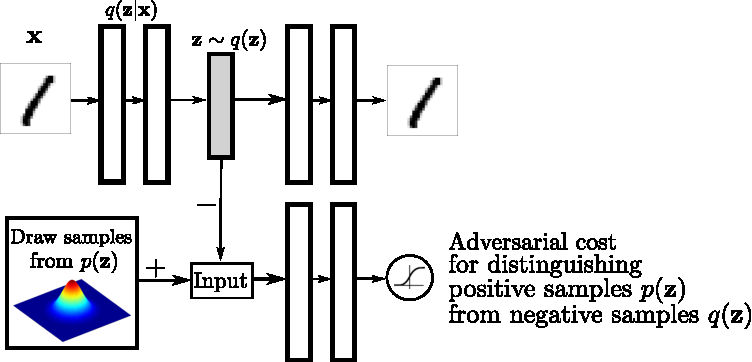
\includegraphics[width=0.8\linewidth]{../images/aae-architecture-01.png}
\end{figure}
\[ p(\vect z) = \int_{\Omega_x} q(\vect z | \vect x) p_d(\vect x) \text d \vect x \]
\end{frame}

\begin{frame}{The encoder}
\begin{itemize}
  \setlength\itemsep{1.5em}
  \item \textbf{Deterministic} — (used in the paper)
  \item \textbf{Gaussian posterior} — $ z_i \sim \Norm(\mu_i(\vect x), \sigma_i(\vect x)) $
  \item \textbf{Universal approximator posterior} — $ \vect z | \vect x, \vect \eta \sim \delta(\vect z - f(\vect x, \vect \eta)) $ \\ where $ \vect \eta $ is random noise with a fixed distribution
  \[ q(\vect z | \vect x) = \int_{\Omega_\eta} q(\vect z | \vect x, \vect \eta) p_\eta(\vect \eta) \text d \vect \eta \]
\end{itemize}
\end{frame}

\begin{frame}{Relationship with VAEs}
VAE aims to minimize the negative ELBO:
\begin{align*}
  \E_{\vect x}[-\log p(\vect x)] 
    &< \E_{\vect x}\left[ \E_{\vect z \sim q(\vect z | \vect x)}[-\log p(\vect x | \vect z)] + \KL(q(\vect z | \vect x) || p(\vect z)) \right] \\
    &= \E_{\vect x}\left[ \E_{\vect z}[-\log p(\vect x | \vect z)] \right] + \E_{\vect x}[- H(q(\vect z | \vect x))] \\ 
    &\qquad + \E_{\vect z \sim q(\vect z | \vect x)}[-\log p(\vect z)] \\
    &= \text{Reconstr. Err.} - \text{Entropy} + \text{Crossentropy}
\end{align*}
\begin{table}
  \begin{tabular}{c c}
    \textbf{VAE} & \textbf{AAE} \\ \hline
  \parbox{0.5\linewidth}{\begin{itemize}
      \item encourages $ q(\vect z) $ to match $ p(\vect z) $ modes because of crossentropy penalty
      \item needs the exact functional form of the prior distribution in order to back-propagate through KL divergence
  \end{itemize}} &
  \parbox{0.45\linewidth}{\begin{itemize}
      \item encourages $ q(\vect z) $ to match the \textit{whole} $ p(\vect z) $ because of the adversarial training
      \item can impose even complicated distributions just through the capability of sampling from them
  \end{itemize}} \\
  \end{tabular}
\end{table}
\end{frame}

\begin{frame}{Relationship with VAE}
\begin{figure}
  \centering
  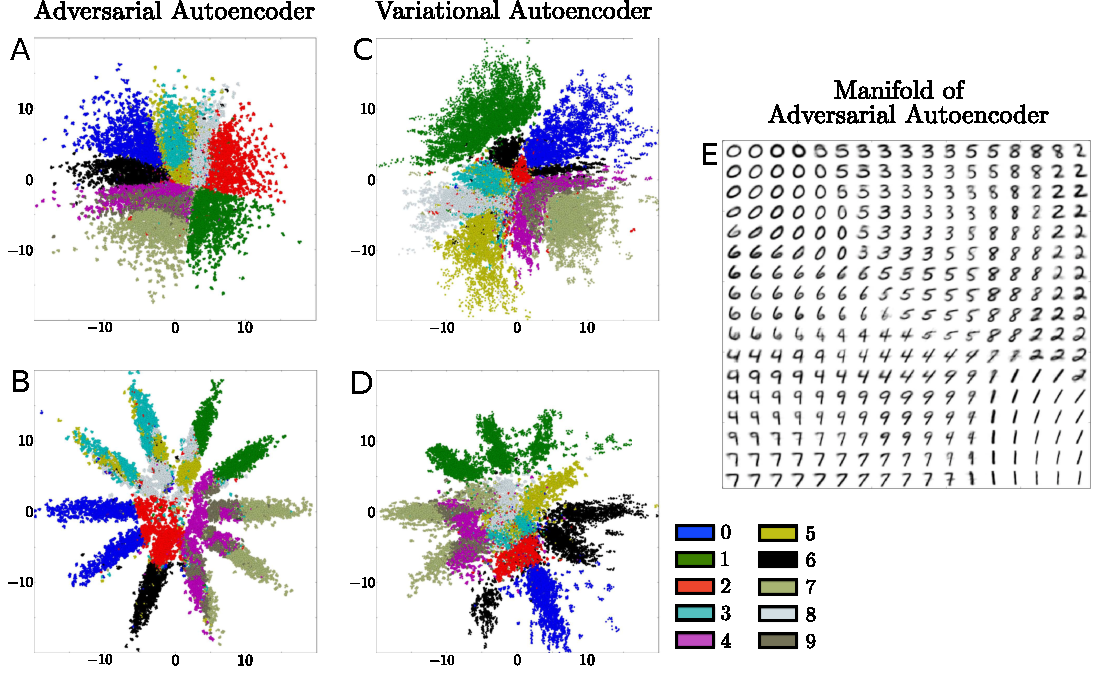
\includegraphics[width=0.8\linewidth]{../images/aae-embedding-01.png}
\end{figure}
\end{frame}

\begin{frame}{Relationship with GAN and GMMN}
\centering
\begin{tabular}{c c}
  \textbf{GAN} & \textbf{AAE} \\ \hline
  \parbox{0.45\linewidth}{\begin{itemize}
      \item imposes the data distribution to the output of a neural network
    \end{itemize}} &
  \parbox{0.45\linewidth}{\begin{itemize}
      \item relies on the autoencoder to capture the data distribution
      \item shapes a much lower dimensional space into a much simpler distribution
    \end{itemize}} \\
  \textbf{GMMN} & \textbf{AAE} \\ \hline
  \parbox{0.45\linewidth}{\begin{itemize}
      \item (first) trains a dropout autoencoder (then) fits a distribution in the code-space of the pretrained network
  \end{itemize}} &
  \parbox{0.45\linewidth}{\begin{itemize}
      \item uses adversarial training as a regularizer that shapes the code distribution while training the autoencoder from scratch
  \end{itemize}}
\end{tabular}
\end{frame}

\begin{frame}{Likelihood analysis}
\begin{itemize}
  \item Benchmarks on: MNIST, \href{../images/tfd.gif}{\underline{Toronto Face Dataset}} (TFD)
  \item Not direct likelihood measure, but lower bound approximation (KDE using Gaussian Parzen window, $ \sigma $ selected by cross-validation)
  \item Samples of 10K and 10M units to estimate the test set log-likelihood
\end{itemize}
\begin{table}
  \centering
  \small
  %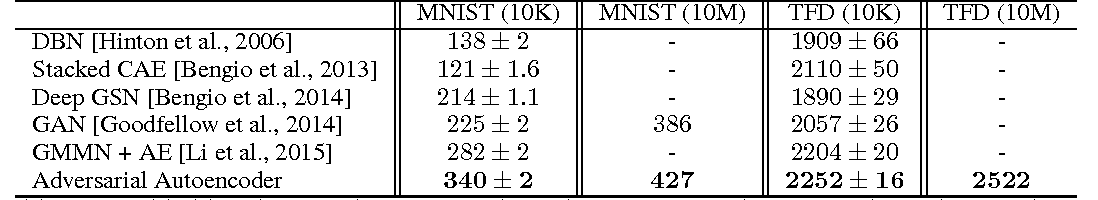
\includegraphics[width=\linewidth]{../images/performance-table-01.png}
  \begin{tabular}{l||c||c||c||c}
    \toprule
                 &   MNIST(10K)    & MNIST(10M) &    TFD(10K)     & TFD(10M) \\ \midrule
    DBN          &  $ 138 \pm 2 $  &     -      & $ 1909 \pm 66 $ &    -     \\
    Stacked CAE  & $ 121 \pm 1.6 $ &     -      & $ 2110 \pm 50 $ &    -     \\
    Deep GSN     & $ 214 \pm 1.1 $ &     -      & $ 2890 \pm 29 $ &    -     \\
    GAN          &  $ 225 \pm 2 $  &  $ 386 $   & $ 2057 \pm 26 $ &    -     \\
    GMMN + AE    &  $ 282 \pm 2 $  &     -      & $ 2204 \pm 20 $ &    -     \\ \midrule
    \textbf{AAE} &  $ 340 \pm 2 $  &  $ 427 $   & $ 2252 \pm 16 $ & $ 2522 $ \\ \bottomrule
  \end{tabular}
\end{table}
\end{frame}

\begin{frame}{Semi-supervised approach}{Architecture}
\begin{itemize}
  \item Incorporate one-hot vector in the latent representation
  \begin{figure}
    \centering
    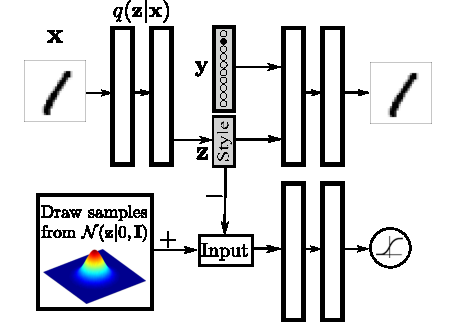
\includegraphics[width=0.6\linewidth]{../images/aae-architecture-02.png}
  \end{figure}
\end{itemize}
\end{frame}

\begin{frame}{Semi-supervised approach}
\begin{itemize}
  \item The AAE disentangles \textit{style} features from \textit{content/semantic} features
  \item Experiments on MNIST and \href{../images/svhn.gif}{\underline{Street View House Number}} dataset (SVHN)
  \begin{figure}
    \centering
    \includegraphics[width=0.6\linewidth]{../images/experiments-supervised-analogy.png}
  \end{figure}
\end{itemize}
\end{frame}

\begin{frame}{Semi-supervised classification}{Architecture}
\begin{tabular}{cl}
  \begin{tabular}{c}
    \hspace{-0.5cm}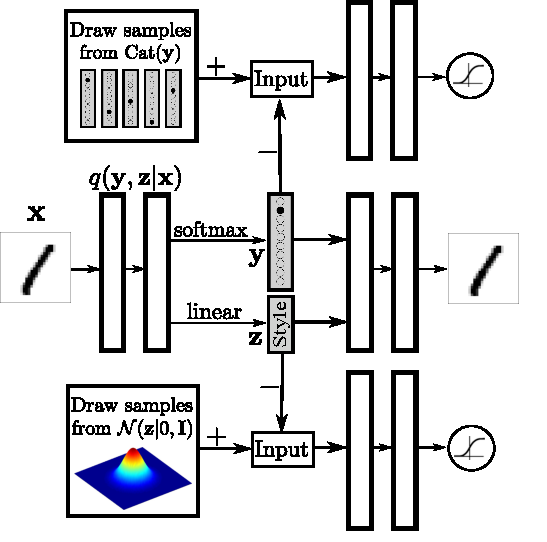
\includegraphics[width=0.45\linewidth]{../images/aae-architecture-03.png}
  \end{tabular} &
  \begin{tabular}{l}
    \hspace{-1cm}\parbox{0.6\linewidth}{% change the width as appropriate
      \begin{itemize}
        \item Improve classification performance using both labeled and unlabeled data
        \item Assume the latent space is a mixed Categorical and Gaussian distribution
        \[ p(\vect y) = \Cat(\vect y) \quad p(\vect z) = \Norm(\vect z; 0, \Id) \]
        \item For each distribution a different adversarial network regularizes the latent representation
    \end{itemize}}
  \end{tabular}
\end{tabular}
\end{frame}

\begin{frame}{Semi-supervised classification}{Training}
3-phase training, all with SGD:
\begin{enumerate}
  \item \textit{reconstruction} — the AE updates the encoder $ q(\vect z, \vect y | \vect x) $ to minimize the reconstruction error
  \item \textit{regularization} — each adversarial network
  \begin{itemize}
    \item first updates the discriminative network to distinguish true samples from the generated samples
    \item then update the encoder to confuse the discriminative networks
  \end{itemize}
  \item \textit{semi-supervised classification} — the AE updates $ q(\vect z, \vect y | \vect x) $ to minimize the cross-entropy cost on a labeled minibatch
\end{enumerate}
\end{frame}

\begin{frame}{Semi-supervised classification}{Results}
\begin{table}
  \centering
  \scriptsize
  %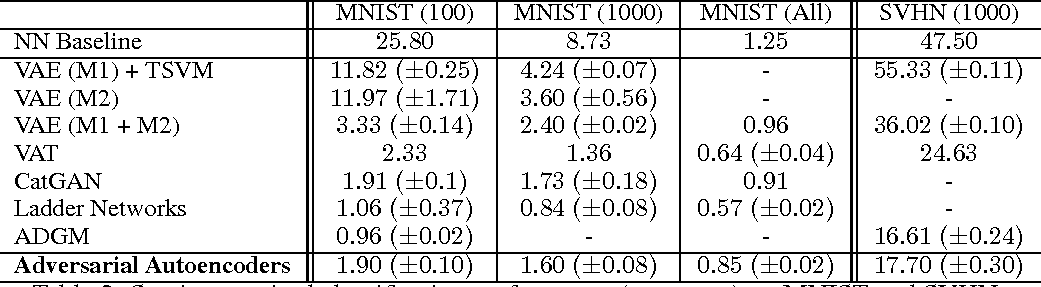
\includegraphics[width=\linewidth]{../images/performance-table-02.png}
    \begin{tabular}{l||c|c|c||c}
    	\toprule
    	                &     MNIST(100)      &    MNIST(1000)    &    MNIST(All)     &     SVHN(1000)     \\ \midrule
    	NN Baseline     &      $ 25.80 $      &     $ 8.73 $      &     $ 1.25 $      &      $ 47.5 $      \\ \midrule
    	VAE (M1) + TSVM & $ 11.82 \pm 0.025 $ & $ 4.24 \pm 0.07 $ &         -         & $ 55.33 \pm 0.11 $ \\
    	VAE (M2)        & $ 11.97 \pm 1.71 $  & $ 3.60 \pm 0.56 $ &         -         & $ 36.02 \pm 0.10 $ \\
    	VAE (M1 + M2)   &  $ 3.33 \pm 0.14 $  & $ 2.40 \pm 0.02 $ &     $ 0.96 $      &     $ 24.63 $      \\
    	CatGAN          &  $ 1.91 \pm 0.1 $   & $ 1.73 \pm 0.18 $ &     $ 0.91 $      &         -          \\
    	Ladder Networks &  $ 1.06 \pm 0.37 $  & $ 0.84 \pm 0.08 $ & $ 0.57 \pm 0.02 $ &         -          \\
    	ADGM            &  $ 0.96 \pm 0.10 $  &         -         &         -         & $ 16.61 \pm 0.24 $ \\ \midrule
    	\textbf{AAE}    &  $ 1.90 \pm 0.10 $  & $ 1.60 \pm 0.08 $ & $ 0.85 \pm 0.02 $ & $ 17.70 \pm 0.30 $ \\ \bottomrule
    \end{tabular}
  \caption{Error rate on semi-supervised classification.}
\end{table}
% AAE models are trained end-to-end while VAE models have to be trained one layer a time
\end{frame}

\begin{frame}{Unsupervised clustering}
\begin{itemize}
  \item Similar to the semi-supervised architecture, but without the semi-supervised training stage
  \item Not necessarily 10 classes, arbitrary number of clusters
  \item Benchmark criterion: find $ \arg\max_{\vect{x}_n} q(y_i | \vect x_n)  $ and assign label of $ x_n $ to all elements of $ i $-th cluster, then compute error rate based on the assigned class labels
\end{itemize}
\begin{table}
  \centering
  \small
  \begin{tabular}{l || c}
    \toprule
                         & MNIST (Unsupervised) \\ \midrule
    CatGAN (20 clusters) & $ 9.70 $             \\
    AAE (16 clusters)    & $ 9.55 \pm 2.05 $    \\
    AAE (30 clusters)    & $ 4.10 \pm 1.13 $    \\ \bottomrule
  \end{tabular}
  \caption{Error-rate on unsupervised clustering}
\end{table}
\end{frame}

\begin{frame}{Unsupervised clustering}
\begin{figure}
  \centering
  \includegraphics[width=0.5\linewidth]{../images/experiments-unsupervised-clusters.png}
\end{figure}
\end{frame}

\begin{frame}{Dimensionality reduction}{Architecture}
\begin{itemize}
  \item Typically, non-regularized autoencoders fracture the manifolds $ \Rightarrow $ very different codes for similar images
  \item Little modification label-integrated AAE architecture
  \begin{figure}
    \centering
    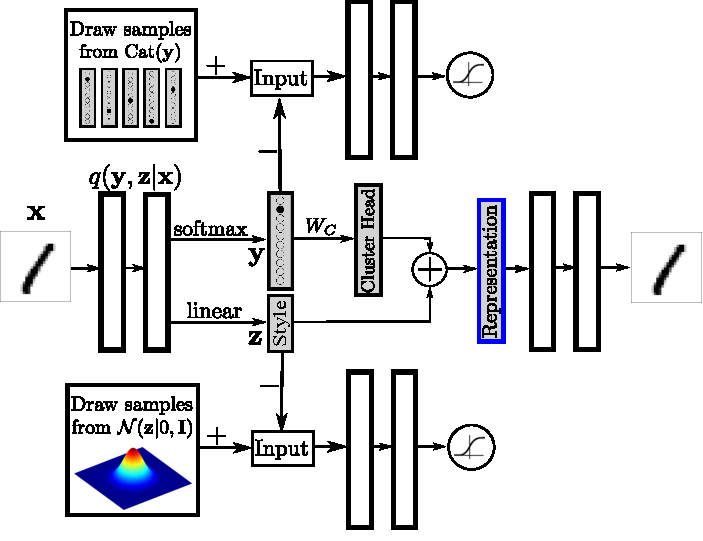
\includegraphics[width=0.6\linewidth]{../images/aae-architecture-04.png}
  \end{figure}
  \item Additional cost to penalize euclidean distance between cluster heads
\end{itemize}
\end{frame}

\begin{frame}{Dimensionality reduction}
\begin{itemize}
  \item Reducing the dimensionality of the hidden space (from 10 to 2) can impact on the predictive power of the whole network
  \item Ad hoc tricks can balance this trade-off
\end{itemize}
\begin{figure}
  \centering
  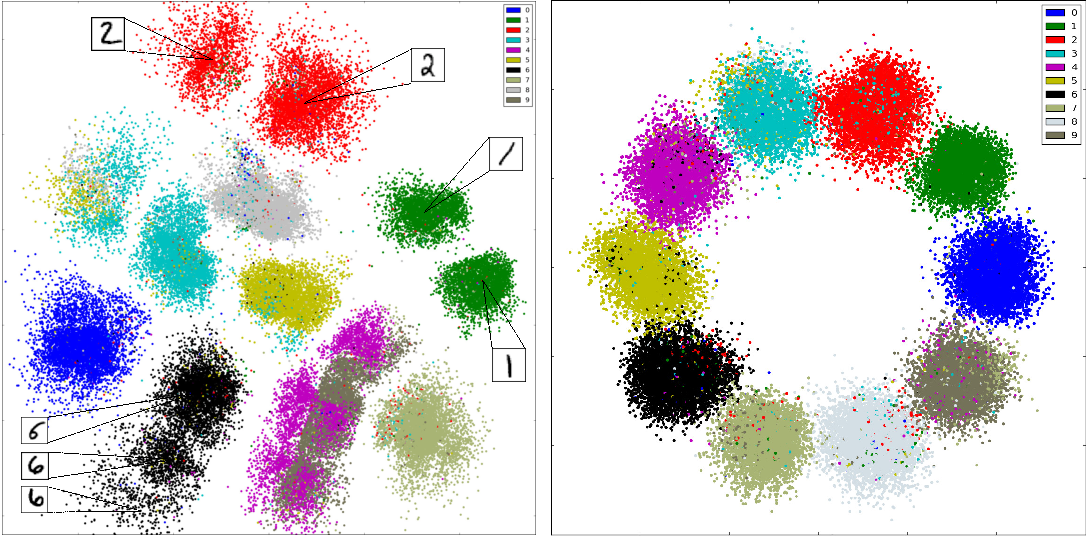
\includegraphics[width=\linewidth]{../images/dim_reduction-scatter-01.png}
\end{figure}
\end{frame}

\begin{frame}{Conclusions}
\textbf{Pros}
\begin{itemize}
  \item it is framework capable of modeling complex distributions only requiring to be able to sample from it
  \item the AAE is highly flexible, could be combined with variational objectives (see \cite{rosca2017variational})
\end{itemize}

\textbf{Cons}
\begin{itemize}
  \item like GANs, it requires much hyper-parameter tuning to perform at the top
  \item it could suffer from complex adversarial game dynamics
  \item it could be an overkill just to treat Gaussian/Gaussian-mixture distributions
\end{itemize}

{\footnotesize * It would need some real-world testing.}
\end{frame}

\begin{frame}{References}
\nocite{bengio2013better}
\nocite{bengio2014deep}
\nocite{goodfellow2014generative}
\nocite{kingma2013auto}
\nocite{maaloe2016auxiliary}
\nocite{li2015generative}

\printbibliography
\end{frame}

\end{document}